\documentclass[12pt, a4paper]{article}
\usepackage[utf8]{inputenc}
\usepackage[spanish]{babel}
\usepackage{csquotes}
\usepackage[style=apa,backend=biber]{biblatex}
\addbibresource{./referencie.bib}
\usepackage[T1]{fontenc}
\usepackage{amsmath}
\usepackage{amsfonts}

\usepackage{amssymb}
\usepackage[a4paper, margin=2.54cm]{geometry}
\usepackage{setspace}
\usepackage{titlesec}
\usepackage{graphicx}
\usepackage{pgfplots}
\usepackage{pgf-pie}
\usepackage{booktabs}
% Configuración de APA 7ma edición

\setlength{\parindent}{0.5in}
\titleformat*{\section}{\normalfont\bfseries}
\titleformat*{\subsection}{\normalfont\bfseries}
\titleformat*{\subsubsection}{\normalfont\bfseries}
\pgfplotsset{compat=1.18}


\begin{document}
\onehalfspacing

\begin{titlepage}
    \begin{center}
        \vspace{0.5in}
        \small “Año del Bicentenario, de la consolidación de nuestra Independencia, y de la conmemoración de las heroicas batallas de Junín y Ayacucho”
  
        
        \LARGE Universidad Nacional Hermilio Valdizan
        
        \Large Facultad de Economía
        
        \vspace{0.5cm}
        
        \begin{figure}[h!]
            \begin{center}
                
\includegraphics[width=0.40\textwidth]{images/unheval.jpg}
                \hspace{0.5cm}  
                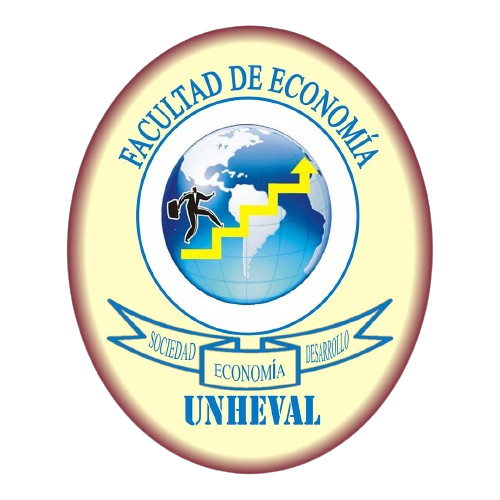
\includegraphics[width=0.45\textwidth]{images/economia.png}
            \end{center}
        \end{figure}
        
        \LARGE{Globalización y su impacto en la economía peruana}
        \vspace{0.5cm}

        \large\textbf{Docente:}

        \large\textbf\author{Cueva Laguna, Jeel E. }

        \large\textbf{Autores:}

        \large\textbf\author{Chuquiyauri Tordecillo, Ronaldhino M.}

        \large\textbf\author{Palomino Ricaldi, Antony R.}        
        
        \vspace{3cm}
        
        \Large Huánuco - Perú 
        
        \large 2024
    \end{center}
\end{titlepage}

\tableofcontents
\newpage

\section{Introducción}

\textbf{Planteamiento del tema}  

La globalización representa uno de los fenómenos más significativos que ha transformado la estructura económica mundial en las últimas décadas \parencite{stiglitz2002}. En el contexto peruano, este proceso ha generado profundas transformaciones en la estructura económica y social del país desde la década de 1990 \parencite{dancourt2016}. Como señalan \textcite{contreras2018} y \textcite{parodi2015}, la integración del Perú a la economía global ha sido un proceso complejo que ha reconfigurado no solo las relaciones comerciales y financieras, sino también el tejido social y productivo del país.

\textbf{Objetivos de la investigación}  

El objetivo principal de esta investigación es analizar el impacto multidimensional de la globalización en la economía peruana, con especial énfasis en el período 1990-2024. Los objetivos específicos incluyen:

\begin{itemize}
    \item Examinar las transformaciones estructurales en la economía peruana como resultado del proceso de globalización .
    \item Evaluar los impactos en las dimensiones comercial, financiera, productiva y socioeconómica.
    \item Identificar las oportunidades y desafíos que presenta la globalización para el desarrollo económico del Perú.
\end{itemize}

\textbf{Justificación del estudio}  

La relevancia de este estudio se fundamenta en la necesidad de comprender las implicaciones de la globalización en la economía peruana, especialmente en un contexto de cambios acelerados y crisis globales. Como argumentan \textcite{mendoza2020} y \textcite{castillo2018}, el análisis de la experiencia peruana en el proceso de globalización proporciona lecciones valiosas para la formulación de políticas públicas y estrategias de desarrollo. Además, \textcite{seminario2019} sostiene que la comprensión de estos impactos es crucial para diseñar políticas que maximicen los beneficios y minimicen los riesgos asociados a la integración global.

\textbf{Metodología empleada}  

La presente investigación adopta un enfoque metodológico cualitativo, de diseño no experimental y nivel explicativo. Se emplea una revisión sistemática de la literatura especializada, análisis de datos estadísticos de fuentes oficiales y estudios de caso específicos. Como señalan \textcite{barrantes2021} y \textcite{lopez2020}, este enfoque permite una comprensión más completa y matizada del fenómeno estudiado. La metodología incluye:

\section{Marco teórico}

\subsection{Conceptualización de la globalización}

\subsubsection{Definiciones principales}
La globalización constituye un fenómeno multidimensional que ha transformado las relaciones económicas, sociales y culturales a nivel mundial. \textcite{held2000} la define como un proceso histórico que altera fundamentalmente los patrones de interacción social y económica mediante la creación de redes transnacionales. Por su parte, \textcite{robertson2003} enfatiza que la globalización representa la intensificación de la conciencia del mundo como un todo, manifestándose en la interconexión de mercados y sociedades.

En el contexto económico, \textcite{krugman2018} y \textcite{sassen2007} coinciden en definir la globalización como un proceso de integración económica caracterizado por el incremento del comercio internacional, los flujos de capital y la movilidad de factores productivos. Esta perspectiva es complementada por \textcite{castells2010}, quien subraya la importancia de las tecnologías de información en la configuración de una economía global interconectada.

\subsubsection{Características fundamentales}
Las características esenciales de la globalización pueden identificarse en múltiples dimensiones. \textcite{dicken2015} señala como elementos fundamentales:
\begin{itemize}
    \item La compresión espacio-temporal de las actividades económicas
    \item La intensificación de los flujos transnacionales
    \item La emergencia de redes globales de producción
    \item La interdependencia de los mercados financieros
\end{itemize}

\textcite{scholte2005} y \textcite{harvey2009} destacan además la desterritorialización de las actividades económicas y la reconfiguración de las relaciones de poder entre estados y mercados como características definitorias del proceso globalizador.

\subsubsection{Dimensiones de la globalización}
El análisis de la globalización requiere una comprensión de sus múltiples dimensiones. \textcite{keohane2018} y \textcite{nye2020} identifican cuatro dimensiones principales:
\begin{itemize}
    \item Económica: Integración de mercados y sistemas productivos
    \item Política: Transformación del rol del Estado y nuevas formas de gobernanza
    \item Social: Cambios en patrones culturales y movilidad humana
    \item Tecnológica: Revolución digital y conectividad global
\end{itemize}

Estas dimensiones, según \textcite{giddens2013}, no operan de manera aislada sino que se retroalimentan mutuamente, generando dinámicas complejas de transformación social y económica.

\subsection{Contexto histórico de la globalización en Perú}

\subsubsection{Antecedentes históricos}
La inserción del Perú en la economía global tiene profundas raíces históricas. \textcite{thorp2012} y \textcite{bulmer1998} identifican distintas etapas en la integración económica del país, desde el período colonial hasta la República. Durante el siglo XX, \textcite{sheahan2001} destaca tres períodos críticos: la era del guano, el período de industrialización por sustitución de importaciones y la apertura económica de los años noventa.

\subsubsection{Proceso de apertura económica}
La apertura económica peruana representa un punto de inflexión en la historia económica del país. \textcite{wise2003} y \textcite{pasco2009} analizan cómo la crisis de los años ochenta precipitó un cambio radical en el modelo económico. Este proceso, según \textcite{gonzales2015}, se caracterizó por:
\begin{itemize}
    \item Liberalización comercial y financiera
    \item Privatización de empresas estatales
    \item Desregulación de mercados
    \item Apertura a la inversión extranjera
\end{itemize}

\subsubsection{Reformas estructurales}
Las reformas estructurales implementadas en la década de 1990 transformaron fundamentalmente la economía peruana. \textcite{abusada2000} y \textcite{parodi2014} documentan las principales reformas:
\begin{itemize}
    \item Reforma comercial y arancelaria
    \item Reforma del sistema financiero
    \item Reforma laboral
    \item Reforma del Estado
\end{itemize}

\textcite{franco2018} y \textcite{vega2019} evalúan el impacto de estas reformas, señalando tanto sus logros en términos de estabilización macroeconómica como sus limitaciones en aspectos de equidad y desarrollo social.

\section{Dimensiones del impacto de la globalización}

\subsection{Dimensión comercial}

La dimensión comercial de la globalización en el Perú ha experimentado una transformación significativa desde la década de 1990. \textcite{santa_cruz2021} y \textcite{rodriguez2019} señalan que esta transformación se caracteriza por una mayor apertura comercial, diversificación de mercados y modernización de la política comercial.

\subsubsection{Evolución del comercio exterior}
El comercio exterior peruano ha mostrado un crecimiento sustancial en las últimas tres décadas. Según \textcite{tello2018}, el valor total del comercio exterior pasó de US\$ 6,700 millones en 1990 a más de US\$ 98,000 millones en 2019, representando un incremento en la ratio de apertura comercial (exportaciones más importaciones sobre PIB) del 22\% al 48\%. Este crecimiento, como señalan \textcite{mendoza2017} y \textcite{torres2020}, se ha caracterizado por:

\begin{itemize}
    \item Un aumento significativo en el volumen de exportaciones tradicionales y no tradicionales
    \item Una diversificación gradual de la canasta exportadora
    \item Un incremento en la participación de las exportaciones no tradicionales
    \item Una mayor integración en las cadenas globales de valor
\end{itemize}

La estructura del comercio exterior ha experimentado cambios significativos. \textcite{leon2019} destaca que mientras en 1990 las exportaciones se concentraban en productos tradicionales (70\%), para 2020 las exportaciones no tradicionales habían aumentado su participación al 30\% del total, evidenciando una diversificación progresiva de la oferta exportable.

\subsubsection{Tratados de libre comercio}
La política comercial peruana ha priorizado la negociación y suscripción de acuerdos comerciales como estrategia de inserción internacional. \textcite{ferrero2018} y \textcite{novak2019} documentan que el Perú ha suscrito más de 20 acuerdos comerciales, entre los que destacan:

\begin{itemize}
    \item El Acuerdo de Promoción Comercial con Estados Unidos (2009)
    \item El Tratado de Libre Comercio con la Unión Europea (2013)
    \item El Acuerdo de Asociación Transpacífico (CPTPP)
    \item Acuerdos bilaterales con China, Japón, Corea del Sur y otros socios asiáticos
    \item Acuerdos regionales en el marco de la Comunidad Andina y la Alianza del Pacífico
\end{itemize}

\textcite{garcia_belaunde2020} y \textcite{morales2021} analizan el impacto de estos acuerdos, señalando que han contribuido a:
\begin{itemize}
    \item Ampliar el acceso a mercados internacionales
    \item Reducir costos de importación de bienes de capital e insumos
    \item Modernizar los marcos regulatorios
    \item Atraer inversión extranjera directa
\end{itemize}

\subsubsection{Diversificación de exportaciones}
La diversificación de las exportaciones representa uno de los desafíos más importantes para la economía peruana. \textcite{alarco2021} identifica patrones significativos en este proceso:

\begin{itemize}
    \item Emergencia de nuevos sectores exportadores no tradicionales
    \item Desarrollo de cadenas de valor en agroindustria y textiles
    \item Incremento en el valor agregado de las exportaciones
    \item Mayor participación en mercados internacionales especializados
\end{itemize}

Sin embargo, \textcite{fairlie2020} señala que persisten desafíos importantes:
\begin{itemize}
    \item Alta concentración en productos primarios
    \item Dependencia de mercados tradicionales
    \item Limitada incorporación de tecnología en procesos productivos
    \item Baja participación en eslabones de alto valor agregado
\end{itemize}

El análisis sectorial realizado por \textcite{sanchez2020} revela que los sectores más dinámicos en términos de diversificación han sido:
\begin{itemize}
    \item Agroexportación no tradicional
    \item Productos pesqueros de valor agregado
    \item Textiles y confecciones
    \item Productos químicos y metalmecánicos
    \item Servicios no financieros
\end{itemize}

\subsection{Dimensión productiva}

La dimensión productiva de la globalización en el Perú ha generado transformaciones significativas en la estructura económica del país. \textcite{tavara2020} señala que estos cambios han afectado tanto la composición sectorial de la producción como los niveles de productividad y competitividad empresarial.

\subsubsection{Transformación de la estructura productiva}
La estructura productiva peruana ha experimentado cambios sustanciales desde la apertura económica. \textcite{jimenez2021} identifica las siguientes transformaciones principales:

\begin{itemize}
    \item Reducción de la participación del sector industrial tradicional
    \item Expansión de los servicios modernos y el comercio
    \item Surgimiento de nuevos clusters productivos
    \item Modernización de sectores tradicionales
\end{itemize}

Sin embargo, \textcite{gonzales2019} señala que esta transformación ha sido heterogénea y presenta las siguientes características:

\begin{enumerate}
    \item Concentración geográfica de la actividad productiva
    \begin{itemize}
        \item 52\% del PIB se genera en Lima y Callao
        \item Persistencia de brechas regionales en productividad
        \item Limitada articulación entre regiones
    \end{itemize}
    
    \item Dualidad estructural
    \begin{itemize}
        \item Coexistencia de sectores modernos y tradicionales
        \item Amplia brecha de productividad entre sectores
        \item Limitada transferencia tecnológica entre segmentos
    \end{itemize}
\end{enumerate}

\subsubsection{Competitividad empresarial}
La globalización ha impuesto nuevos desafíos en términos de competitividad empresarial. \textcite{torres2021} analiza los principales aspectos:

\begin{itemize}
    \item Mejoras en la gestión empresarial
    \begin{itemize}
        \item Adopción de estándares internacionales
        \item Implementación de sistemas de calidad
        \item Modernización de procesos administrativos
    \end{itemize}
    
    \item Desarrollo de cadenas de valor
    \begin{itemize}
        \item Integración con proveedores globales
        \item Especialización productiva
        \item Certificaciones internacionales
    \end{itemize}
\end{itemize}

No obstante, \textcite{villarreal2019} identifica importantes limitaciones:
\begin{itemize}
    \item Alta informalidad empresarial (70\% de empresas)
    \item Baja productividad laboral
    \item Limitado acceso a financiamiento
    \item Escasa inversión en investigación y desarrollo
\end{itemize}

\subsubsection{Innovación y tecnología}
El proceso de globalización ha evidenciado la importancia crítica de la innovación y la tecnología. \textcite{sagasti2020} analiza la situación del Perú en este ámbito:

\begin{itemize}
    \item Inversión en I+D
    \begin{itemize}
        \item 0.12\% del PIB (2020)
        \item Principalmente financiada por el sector público
        \item Concentrada en investigación básica
    \end{itemize}
    
    \item Adopción tecnológica
    \begin{itemize}
        \item Predominio de tecnologías importadas
        \item Limitada capacidad de adaptación
        \item Baja generación de patentes
    \end{itemize}
\end{itemize}

\textcite{peters2021} identifica las principales barreras para la innovación:
\begin{itemize}
    \item Limitada vinculación academia-empresa
    \item Escasez de capital humano especializado
    \item Débil infraestructura tecnológica
    \item Marco institucional insuficiente
\end{itemize}

Sin embargo, \textcite{loayza2019} destaca algunas experiencias exitosas:
\begin{itemize}
    \item Desarrollo de startups tecnológicas
    \item Innovaciones en el sector agroindustrial
    \item Modernización de servicios financieros
    \item Adopción de tecnologías digitales
\end{itemize}

\subsection{Dimensión Socioeconómica}

\subsubsection{Empleo y mercado laboral}
La globalización ha transformado significativamente la estructura del mercado laboral peruano. Según \textcite{chacaltana2016formalizacion}, el proceso de apertura económica generó una recomposición del empleo entre sectores, con un incremento del empleo formal en sectores vinculados al comercio internacional y una reducción en sectores tradicionalmente protegidos. \textcite{yamada2021labor} señala que la flexibilización laboral implementada durante los años noventa facilitó la creación de empleo en el sector formal, aunque también incrementó la temporalidad de los contratos laborales.

La calidad del empleo ha mostrado tendencias mixtas. \textcite{lavado2018efectos} documenta que los sectores más expuestos a la competencia internacional han experimentado mejoras en las condiciones laborales y salarios, mientras que \textcite{rodriguez2019informalidad} encuentra que la persistencia de altos niveles de informalidad laboral (cercana al 70\% de la PEA) ha limitado los beneficios de la globalización en términos de protección social y derechos laborales.

\subsubsection{Distribución del ingreso}
El impacto de la globalización en la distribución del ingreso en Perú ha sido objeto de intenso debate académico. \textcite{webb2019peru} argumenta que el crecimiento económico impulsado por la apertura comercial contribuyó a reducir la pobreza monetaria de 58.7\% en 2004 a 20.2\% en 2019. Sin embargo, \textcite{mendoza2020desigualdad} señala que la desigualdad de ingresos, medida por el coeficiente de Gini, ha mostrado una rigidez a la baja, manteniéndose en niveles elevados para estándares internacionales.

Las brechas regionales también han sido significativas. \textcite{escobal2018geografia} documenta que las regiones más integradas a los mercados internacionales han experimentado mayores reducciones en sus niveles de pobreza, mientras que \textcite{barrantes2019disparidades} encuentra que las zonas rurales y con menor conectividad han quedado rezagadas en términos de ingresos y acceso a servicios básicos.

\subsubsection{Desarrollo social}
La globalización ha tenido efectos heterogéneos en el desarrollo social del Perú. \textcite{vasquez2020inclusion} destaca mejoras significativas en indicadores de desarrollo humano como el acceso a educación y salud, atribuibles en parte a la mayor disponibilidad de recursos fiscales generados por el crecimiento económico. Por su parte, \textcite{franco2019vulnerabilidad} señala que la clase media emergente, beneficiada por el proceso de globalización, se mantiene vulnerable a choques económicos externos.

El acceso a servicios públicos de calidad continúa siendo un desafío. \textcite{sanchez2021servicios} encuentra que, si bien la cobertura de servicios básicos se ha expandido, persisten brechas importantes en la calidad de estos servicios entre zonas urbanas y rurales. \textcite{aramburú2019cohesion} argumenta que la globalización ha contribuido a profundizar las diferencias en el acceso a oportunidades de desarrollo entre distintos grupos socioeconómicos.

\section{Análisis de Impactos}

\subsection{Oportunidades y Beneficios}

\textbf{Crecimiento económico}
La integración de Perú en la economía global ha generado un impacto significativo en el crecimiento económico del país. \textcite{dancourt2018boom} documenta que durante el período 2002-2013, el país experimentó un crecimiento promedio anual del PBI de 6.1\%, impulsado principalmente por el boom de commodities y la expansión del comercio internacional. \textcite{castillo2020exportaciones} complementa este análisis señalando que la diversificación de mercados de exportación permitió mantener tasas de crecimiento positivas incluso durante períodos de volatilidad internacional.

El fortalecimiento de los fundamentos macroeconómicos ha sido otro beneficio notable. Según \textcite{velarde2019politica}, la disciplina fiscal y monetaria adoptada como parte del proceso de inserción internacional ha contribuido a mantener la estabilidad de precios y tipo de cambio. \textcite{pastor2021reservas} destaca que la acumulación de reservas internacionales ha fortalecido la capacidad del país para enfrentar choques externos.

\textbf{Modernización productiva}
La exposición a la competencia internacional ha catalizado la modernización del aparato productivo peruano. \textcite{tello2019productividad} encuentra que los sectores más expuestos al comercio internacional han experimentado incrementos significativos en su productividad total de factores. Por su parte, \textcite{garcia2020innovacion} documenta que la inversión extranjera directa ha facilitado la transferencia de tecnología y conocimientos, particularmente en sectores como minería, agroindustria y manufactura.

La adopción de estándares internacionales ha sido otro vector de modernización. \textcite{kuramoto2018cadenas} señala que la participación en cadenas globales de valor ha incentivado la adopción de certificaciones y mejores prácticas productivas. \textcite{távara2021calidad} complementa este análisis destacando el desarrollo de sistemas de gestión de calidad en empresas exportadoras.

\textbf{Acceso a mercados}
La red de acuerdos comerciales ha expandido significativamente las oportunidades de mercado para las empresas peruanas. \textcite{ferrero2019tlc} documenta que los TLC han permitido acceder a mercados que representan más del 80\% del PBI mundial. \textcite{malca2020pymes} encuentra que incluso las pequeñas y medianas empresas han logrado insertarse en nichos específicos del mercado internacional.

El desarrollo de la infraestructura logística, aunque aún insuficiente, ha facilitado el aprovechamiento de estas oportunidades. \textcite{bonifaz2021infraestructura} señala mejoras significativas en puertos y aeropuertos, mientras que \textcite{rosales2019conectividad} destaca la importancia de continuar reduciendo los costos logísticos para maximizar los beneficios del acceso a mercados.

\subsection{Desafíos y Riesgos}

\textbf{Vulnerabilidad externa}  

La mayor integración internacional ha incrementado la exposición de la economía peruana a choques externos. \textcite{mendoza2021volatilidad} analiza cómo la dependencia de las exportaciones de materias primas genera vulnerabilidad ante fluctuaciones en los precios internacionales. \textcite{jimenez2020ciclos} complementa este análisis documentando la correlación entre los ciclos económicos peruanos y las condiciones financieras globales.

Los flujos de capital volátil representan otro factor de riesgo. \textcite{rossini2019politica} señala que los sudden stops y reversiones en los flujos de capital pueden generar presiones sobre el tipo de cambio y el sistema financiero. \textcite{cruz2021financiera} argumenta que la dolarización parcial de la economía amplifica estos riesgos.

\textbf{Desigualdad y brechas sociales}  

La globalización ha tenido efectos heterogéneos en la distribución de beneficios. \textcite{herrera2020brechas} encuentra que las regiones con menor dotación de capital humano y físico han quedado rezagadas en el proceso de integración internacional. \textcite{yamada2021movilidad} documenta que la movilidad social intergeneracional sigue siendo limitada a pesar del crecimiento económico.

Las brechas de productividad entre sectores se han ampliado. \textcite{chacaltana2019dualidad} analiza la persistencia de un sector informal significativo que opera con baja productividad y limitado acceso a tecnología. \textcite{lavado2020skills} señala que la brecha de habilidades limita el aprovechamiento de oportunidades generadas por la globalización.

\textbf{Sostenibilidad ambiental}  

La presión sobre los recursos naturales se ha intensificado con la integración internacional. \textcite{glave2021extractivas} documenta los impactos ambientales asociados a la expansión de industrias extractivas orientadas a la exportación. \textcite{pulgar2019conflictos} analiza cómo esta presión ha generado conflictos socioambientales en diversas regiones del país.

El cambio climático representa un desafío adicional. \textcite{vargas2020clima} señala la vulnerabilidad de sectores exportadores clave, como la agroindustria, ante eventos climáticos extremos. \textcite{sanchez2021adaptacion} enfatiza la necesidad de incorporar consideraciones de sostenibilidad en la estrategia de desarrollo del país.

\section{Conclusiones}


\textbf{Síntesis de hallazgos}  

La experiencia peruana con la globalización presenta un balance mixto con importantes lecciones. \textcite{seminario2022balance} señala que el proceso de apertura económica generó una transformación estructural de la economía peruana, con resultados positivos en términos de crecimiento económico y reducción de la pobreza monetaria. Sin embargo, \textcite{paz2021desafios} argumenta que esta transformación no ha sido suficiente para superar problemas estructurales como la informalidad y la desigualdad regional.

La evidencia analizada sugiere que los beneficios de la globalización han sido heterogéneos. \textcite{vega2021disparidades} encuentra que las regiones y sectores con mayores ventajas competitivas iniciales y mejor infraestructura han capitalizado más efectivamente las oportunidades del comercio internacional. Por su parte, \textcite{torres2020vulnerabilidad} documenta que la exposición a choques externos ha incrementado la volatilidad macroeconómica, aunque el fortalecimiento del marco institucional ha mejorado la capacidad de respuesta del país.

\textbf{Tendencias identificadas}  

El análisis revela patrones importantes en la evolución de la economía peruana. \textcite{parodi2021tendencias} identifica una correlación positiva entre la profundización de la integración internacional y la modernización del aparato productivo nacional. \textcite{contreras2022perspectivas} señala que las empresas exportadoras muestran consistentemente mayores niveles de productividad y adopción tecnológica que aquellas orientadas exclusivamente al mercado interno.

No obstante, persisten desafíos significativos. \textcite{jimenez2021brechas} documenta la persistencia de brechas de productividad entre sectores económicos y regiones geográficas. \textcite{gonzales2022sostenibilidad} enfatiza la necesidad de equilibrar los objetivos de crecimiento económico con la sostenibilidad ambiental y la cohesión social.
\newpage
\printbibliography
\end{document}